\documentclass[12pt]{article}

\usepackage{discrete}

\def\thetitle{Introduction to Graph Theory} % will be put in the center header on the first page only.
\def\lefthead{Math 228 Notes} % will be put in the left header
\def\righthead{\thetitle} % will be put in the right header



\begin{document}


\section{Coloring}

\begin{activity}
Mapmakers in the fictional land of Euleria have drawn the borders of the various dukedoms of the land.  Now to make the map pretty, they wish to color each region.  Adjacent regions must be colored differently, but it is perfectly fine to color two distant regions with the same color.  What is the fewest colors the mapmakers can use and still accomplish this task?

\begin{center}
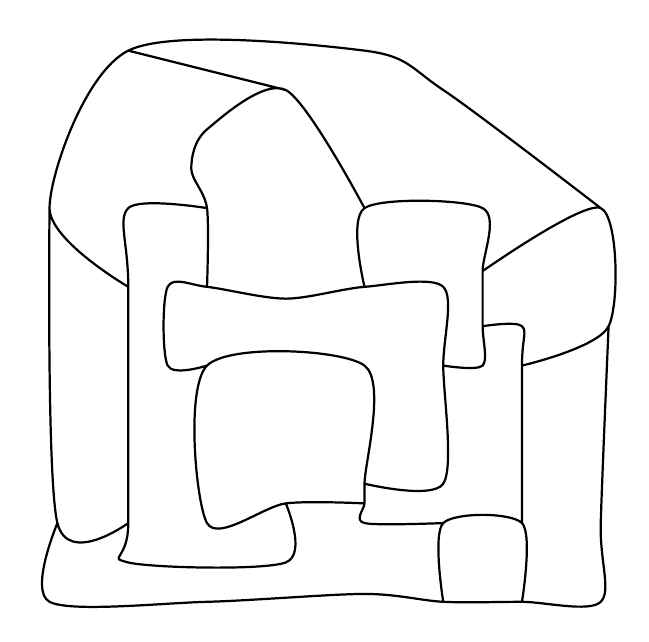
\begin{tikzpicture}
\draw[thick] 
	plot [smooth] coordinates {(0.1,1) (0,0) (2,0) (4,0.1) (5,0) (6,0) (7,0) (7,1) (7.1,3.5)}
	plot [smooth] coordinates {(1,1) (0.1,1) (0,5)} 
	plot [smooth] coordinates {(2,5) (1,5) (1,4) (1,1) (1,.5) (3,.5) (3,1.25)}
	plot [smooth] coordinates {(5,0) (5,1) (6,1) (6,0)}
	plot [smooth] coordinates {(6,1) (6,3) (6,3.5) (5.5,3.5)}
	plot [smooth] coordinates {(5,1) (4,1) (4,1.25) (4,1.5) (4,3) (2,3) (2,1) (3,1.25) (4,1.25)}
	plot [smooth] coordinates {(4,1.5) (5,1.5) (5,3) (5,4) (4,4) (3,3.85) (2,4) (1.5,4) (1.5,3) (2,3)}
	plot [smooth] coordinates {(5,3) (5.5,3) (5.5,3.5) (5.5, 4.2) (5.5,5) (4,5) (4,4)}
	plot [smooth] coordinates {(6,3) (7.1, 3.5) (7,5) (5.5,4.2)}
	plot [smooth] coordinates {(7,5) (5,6.5) (4,7) (1,7) (0,5) (1,4)}
	plot [smooth] coordinates {(2,4) (2,5) (1.8,5.5) (2,6) (3,6.5) (4,5)}
	plot [smooth] coordinates {(1,7) (3,6.5)};
\end{tikzpicture}
\end{center}

\end{activity}

Perhaps the most famous graph theory problem is how to color maps.  

\begin{quote}
  \textbf{Question:} Given any map of countries, states, counties, etc. how many colors are needed to color each region on the map so that neighboring regions are colored differently?
\end{quote}

Actual map makers usually use around seven colors - for one thing, they require watery regions to be a specific color, and with a lot of colors it is easier to find a permissible coloring.  But we want to know whether there is a smaller palette that will work for any map.

How is this related to graph theory?  Well, if we place a vertex in the center of each region (say in the capital of each state) and then connect two vertices if their states share a border, we get a graph.  The coloring regions on the map corresponds to coloring the vertices of the graph.  Since neighboring regions cannot be colored the same, our graph cannot have vertices colored the same when those vertices are adjacent (connected by an edge).

In general, given any graph, a coloring of the vertices is called (not surprisingly) a {\em vertex coloring}.  If the vertex coloring has the property that adjacent vertices are colored differently, then the coloring is called {\em proper}.  Every graph has a proper vertex coloring - for example, you could color every vertex with a different color.  But often you can do better.  The smallest number of colors needed to get a proper vertex coloring is called the {\em chromatic number} of the graph.

\begin{example}
  Find the chromatic number of the graphs below.
  \begin{center}
    \hfill
    \begin{tikzpicture}
      \foreach \x in {0,...,6}
      \draw[thick] (\x*60:1) \v -- (\x*60+60:1) -- (\x*60+180:1) -- cycle;
    \end{tikzpicture}
    \hfill
    \begin{tikzpicture}[yscale=.8]
      \draw[thick] (-1,0) \v -- (0,0) \v -- (1,0) \v -- (.5,1) \v -- (0,0) -- (-.5,1) \v -- (0,2) \v -- (.5,1) -- (-.5,1) -- (-1,0);
    \end{tikzpicture}
    \hfill
    \begin{tikzpicture}[yscale=.8, xscale=1.5]
 \draw[thick] (-1, 0) \v -- (-.5,2) \v -- (0,0) \v -- (.5, 2) \v -- (1,0) \v -- (-.5,2) (.5,2) -- (-1,0);
  \end{tikzpicture}
  \hfill ~
  \end{center}

\begin{solution}
  The graph on the left is $K_6$.  The only way to properly color the graph is to give every vertex a different color (since every vertex is adjacent to every other vertex).  Thus the chromatic number is 6.
  
  The middle graph can be properly colored with just 3 colors (Red, Blue, and Green).  For example:
  
  \begin{center}
        \begin{tikzpicture}[yscale=.8]
      \draw[thick] (-1,0) \vb{R} -- (0,0) \vb{B} -- (1,0) \vb{G} -- (.5,1) \vr{R} -- (0,0) -- (-.5,1) \vl{G} -- (0,2) \va{B} -- (.5,1) -- (-.5,1) -- (-1,0);
    \end{tikzpicture}
  \end{center}
  
  There is no way to color it with just two colors, since there are three vertices mutually adjacent (i.e., a triangle).  Thus the chromatic number is 3.
  
  The graph on the right is just $K_{2,3}$.  As with all bipartite graphs, this graph has chromatic number 2 - color the vertices in the top row red and the vertices on the bottom row blue.
\end{solution}

\end{example}

It appears that graphs can have any chromatic number.  It should not come as a surprise that $K_n$ has chromatic number $n$.  So how could there possibly be an answer to the original map coloring question?  If the chromatic number of graph can be arbitrarily large, then it seems like there would be no upper bound to the number of colors needed for any map.  But there is.

The key observation is that while it is true that for any number $n$, there is a graph with chromatic number $n$, only some graphs arrive as representations of maps.  If you convert a map to a graph, the edges between vertices correspond to borders between the countries.  So you should be able to connect vertices in such a way where the edges do not cross.  In other words, the graphs representing maps are all {\em planar}!

So the question is, what is the larges chromatic number of any planar graph?  The answer is one of the best know theorems of mathematics:

\begin{theorem}[The Four Color Theorem]
If $G$ is a planar graph, then the chromatic number of $G$ is less than or equal to 4.  Thus any map can be colored with 4 or fewer colors.
\end{theorem}

We will not prove this theorem.  Really.  Even though the theorem is easy to state and understand, the proof is not.  In fact, there is currently no ``easy'' known proof of the theorem.  The current best proof still requires powerful computers to check an {\em unavoidable set} of  633 {\em reducible configurations}.  The idea is that every graph must contain one of these reducible configurations (this fact also needs to be checked by a computer) and that reducible configurations can in fact be colored in 4 or fewer colors. 


\subsection{Coloring in General}
\begin{activity}
The math department plans to offer 10 classes next semester.  Some classes cannot run at the same time (perhaps they are taught by the same professor, or are required for seniors).  

\begin{center}
\begin{tabular}{cl}
\textbf{Class:} & \textbf{Conflicts with:} \\ \hline
A & D I \\
B & D I J \\
C & E F I \\
D & A B F \\
E & H I\\
F & I\\
G & J \\
H & E I J\\
I & A B C E F H \\
J & B G H
\end{tabular}
\end{center}

How many different time slots are needed to teach these classes (and which should be taught at the same time)?  More importantly, how could we use graph coloring to answer this question?
\end{activity}


Cartography is certainly not the only application of graph coloring.  There are plenty of situations in which you might wish partition the objects in question so that related objects are not in the same partition.  In addition to scheduling problems like the one above, here are a couple of further examples.

\begin{example}
Radio stations broadcast their signal at certain frequencies.  However, there are a limited number of frequencies to choose from, so nationwide many stations use the same frequency.  This works because the stations are far enough apart that their signals will not interfere; no one radio could pick them up at the same time.

Suppose 10 new radio stations are to be set up in a currently unpopulated (by radio stations) region.  The radio stations that are close enough to each other to cause interference are recorded in the table below.  What is the fewest number of frequencies the stations could use.



\begin{solution}


\end{solution}
\end{example}\todo[inline]{create table of stations - we want chromatic number at least 5.}
\todo[inline]{write solution}
\begin{example}
Your high school chemistry teacher is getting a new lab.  She will need cabinets to store various chemicals.  To avoid explosions, it is important that some pairs of chemicals are definitely not stored in the same cabinet.   What is the fewest number of cabinets the chemist can use to store these chemicals?

\begin{solution}

\end{solution} 
\end{example}
\todo{give list of conflicting chemicals} \todo[inline]{write solution}
Notice that in the first example, the chromatic number was 5.  This is not a counter-example to the Four Color Theorem, since the graph representing the radio stations is not planar.  It would be nice to have some quick way to find the chromatic number of a (possibly non-planar) graph.  It turns out nobody knows whether an efficient algorithm for computing chromatic numbers exists.  

Not all hope is lost however.  While we might not be able to find the exact chromatic number of graph easily, we can often give a reasonable range for the chromatic number.  In other words, we can give upper and lower bounds for chromatic number.

This is actually not very difficult: for every graph $G$, the chromatic number of $G$ is at least 1 and at most the number of vertices of $G$.  

What?  You want \emph{better} bounds on the chromatic number?  Well you are in luck.

A \emph{clique} in a graph is a set of vertices all of which are pairwise adjacent.  In other words, a clique of size $n$ is just a copy of the complete graph $K_n$.  We define the \emph{clique number} of a graph to be the largest $n$ for which the graph contains a clique of size $n$.  Now any clique of size $n$ cannot be colored with fewer than $n$ colors, so we have a nice lower bound:

\begin{theorem}
The chromatic number of a graph $G$ is at least the clique number of $G$.
\end{theorem}

There are times when the chromatic number of $G$ is \emph{equal} to the clique number.  These graphs have a special name -- they are called \emph{perfect}.  If you know that a graph is perfect, then finding the chromatic number is simply a matter of searching for the largest clique.\footnote{There are special classes of graphs which can be proved to be perfect.  One such class is the set of \emph{chordal} graphs, which have the property that every cycle in the graph contains a \emph{chord} -- an edge between two vertices in of the cycle which are not adjacent in the cycle.}  However, not all graphs are perfect.  

For an upper bound, it is also possible to do better than just the number of vertices.  One reasonable guess would be to say that the chromatic number is never more than the largest degree of any vertex in the graph.  This seems reasonable, because\ldots\todo{does it?}.  This is almost true, and is a result known as Brooke's Theorem.

\todo[inline]{state Brooke's theorem}



%\begin{activity}
%A \emph{proper vertex coloring} of a graph is a coloring in which no two adjacent vertices are colored the same color.  The \emph{chromatic number} of a graph is the smallest number of colors needed for a proper coloring of the graph.
%
%For each graph below, find a proper coloring and determine the chromatic number of the graph.  As you are working on these colorings, think about the following ideas:
%\begin{enumerate}
%\item Before I even start coloring the graph, can I come up with an upper bound on the number of colors I will need (a bound that is better than simply the total number of vertices in the graph)? 
%
%\item Before I even start coloring the graph, can I come up with a lower bound on the number of colors I will need (a bound that is better than simply 2)?  
%
%\item Once you have colored the graph, make sure that you check your coloring with your tablemates to try to determine if you used the minimal number of colors.  Talk with each other about reasons why you couldn't have used fewer colors than you did.
%  
%\item For each graph, try to identify if it is a type of graph that we've talked about before (i.e.\ does it have a special name or special properties).  If the graph is a named graph, try to see if you can generalize the ideas you used in your coloring of this graph to other graphs of that same type.
%\end{enumerate}
%
%ADD GRAPHS!
%
%\end{activity}\todo{Replace this with a map coloring question}
\todo[inline]{Finish up this section.  Put in some exercises about finding graphs which are not perfect.}


\subsection{Coloring Edges}

\todo[inline]{MAYBE ADD VIZINGS THEOREM and an application.  Then transition to Ramsey theory}

The chromatic number of a graph tells us about coloring vertices - but we could also ask about coloring edges.  What if we colored every edge of a graph either red or blue.  Can we do so without, say, creating a triangle of same like colored edges (i.e., an all red or all blue triangle - we say the triangle is {\em mono-chromatic})?  Certainly for some graphs the answer is yes - try doing so for $K_4$.  What about $K_5$?  $K_6$?  How far can we go?  

The answer the above problem is known - I encourage you to try to solve it.  We could extend the question though - what if we had three colors?  What if we were trying to avoid other graphs.  The surprising fact is that very little is known about these questions.  For example, we know that you need to go up to $K_{17}$ in order to force a mono-chromatic triangle using three colors, but nobody knows how big you need to go with more colors.  Similarly, we know that using two colors $K_{18}$ is the smallest graph that forces a mono-chromatic copy of $K_4$, but the best we have to force a mono-chromatic $K_{5}$ is a range - somewhere from $K_{43}$ to $K_{49}$.


\end{document}


